\documentclass[12pt]{article}
\usepackage[nottoc]{tocbibind}
\usepackage[parfill]{parskip}
\usepackage{graphicx}
% \graphicspath{ {image/} }
\usepackage{geometry}
 \geometry{
 a4paper,
 total={170mm,257mm},
 left=20mm,
 top=20mm,
 }
\usepackage[
backend=biber,
style=ieee,
citestyle=numeric
]{biblatex}
\usepackage{listings}
\usepackage{color}

\definecolor{codegreen}{rgb}{0,0.6,0}
\definecolor{codegray}{rgb}{0.5,0.5,0.5}
\definecolor{codepurple}{rgb}{0.58,0,0.82}
\definecolor{backcolour}{rgb}{0.95,0.95,0.92}

\lstdefinestyle{mystyle}{
    backgroundcolor=\color{backcolour},
    commentstyle=\color{codegreen},
    keywordstyle=\color{magenta},
    numberstyle=\tiny\color{codegray},
    stringstyle=\color{codepurple},
    basicstyle=\footnotesize,
    breakatwhitespace=false,
    breaklines=true,
    captionpos=b,
    keepspaces=true,
    numbers=left,
    numbersep=5pt,
    showspaces=false,
    showstringspaces=false,
    showtabs=false,
    tabsize=2
}

\lstset{style=mystyle}
\usepackage[]{algorithm2e}
\usepackage{CJKutf8}
\usepackage{amsmath}
% \makeatletter
% \setlength{\@fptop}{0pt}
% \setlength{\@fpbot}{0pt plus 1fil}
% \makeatother
\addbibresource{biblio.bib}

\renewcommand{\baselinestretch}{1.5}
\renewcommand*\contentsname{TABLE OF CONTENTS}


\begin{document}

\begin{titlepage}
\begin{center}
        \vspace*{3cm}
        {\Huge A Question Answering System on SQuAD Dataset Using an End-to-end Neural Network}\\

        \vspace*{3cm}
        {\Huge CS297 Report}\\

        \vspace{3 cm}
        Student: Bo Li\\
        Advisor: Dr. Chris Pollett\\
        Date: Dec 2017

 \end{center}
\clearpage
\end{titlepage}

\begin{titlepage}
\tableofcontents
\clearpage
\end{titlepage}



\section{Introduction}

Question Answering(QA) is about making a computer program that could answer questions in natural language automatically. QA techniques are widely used among search engines, personal assistant applications on smart phones, voice control systems and a lot more other applications. In recent years, more end-to-end neural network architectures are built to do question answering tasks. In contrast, traditional solutions use syntactic and semantic analyses and hand made features. End-to-end neural network approach gives more accurate result. However, traditional ways are more explainable. The Stanford Question Answering Dataset (SQuAD) is used in this project. It includes questions asked by human beings on Wikipedia articles. The answer to each question is a segment of the corresponding Wikipedia article\cite{rajpurkar2016squad}. In total, SQuAD contains 100,000+ question-answer pairs on 500+ articles\cite{rajpurkar2016squad}. The goal of this project is to build a QA system on SQuAD using an end-to-end neural network architecture.

This report is about my progress in CS297. Section \ref{sec:calculation}  corresponds to deliverable 1, which is a study on the mathematical basis of neural network. Section \ref{sec:embdding} corresponds to Deliverable 2, in which I did word embedding of Chinese classic poems. Section \ref{sec:setup} and Section \ref{sec:implementpaper} correspond to Deliverable 3 and 4, which include setting up development infrastructure, understanding model, and designing implementation architecture for my QA system. Section \ref{sec:summary} summarizes my work in CS297 and proposes future work in CS298.



\section{Calculation of Back Propagation}\label{sec:calculation}

The purpose of this deliverable is to understand the mathematical basis of neural networks. This is important since a neural network model will be used to build my QA system. I fulfilled the purpose by doing back propagation on a dummy feed forward neural network example.


Define the model as
$$\hat{y}=softmax(z_2)$$
$$z_2=h\cdot W_2 + b_2$$
$$h=sigmoid(z_1)$$
$$z_1=x\cdot W_1+b_1$$

Define the loss as
$$J(W_1, b_1, W_2, b_2, x, y)$$
$$=cross\_entropy(y, \hat{y})$$
$$=-\frac{1}{D_y}\sum_{i=1}^{D_y}y_i \times \log{\hat{y_i}} $$

After using chain rules multiple times, I got

$$\frac{dJ}{dz_2}=\hat{y} - y$$
$$\frac{dJ}{db_2}=\frac{dJ}{dz_2}$$
$$\frac{dJ}{dh}=\frac{dJ}{dz_2}\cdot W_2^T$$
$$\frac{dJ}{dW_2}=h^T \cdot \frac{dJ}{dz_2}$$

By working out this dummy example, I got a solid foundation of back propagation and became more prepared for understanding more complex neural network models.



\section{Implementation of Word Embedding}\label{sec:embdding}

\begin{figure}[h]
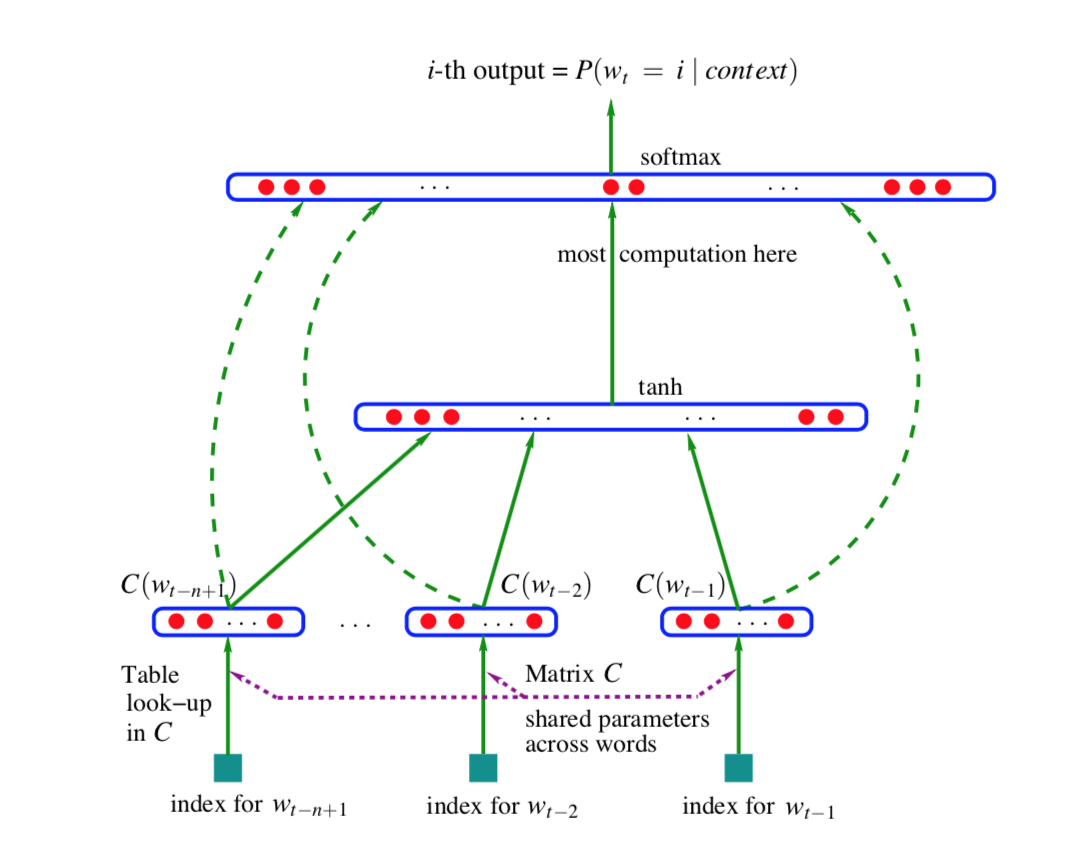
\includegraphics[width=15cm, height=10cm]{image/nplm_architecture.png}
\centering
\caption{Neural architecture: $f(i,w_{t-1},... ,w_{t-n+1}) =g(i,C(w_{t-1}),... ,C(w_{t-n+1}))$ where $g$ is the neural network and $C(i)$ is the $i$-th word feature vector\cite{bengio2003neural}}
\label{fig:nplm}
\end{figure}

Word embedding is an important language modeling technique. It is usually the first step towards applying neural networks to natural language processing. Understanding word embedding is an essential part of understanding how to use a neural network model to build a QA system.

Word embedding is a way to map each word to a feature vector in a continuous space. The dimension of the continuous space is much lower than the dimension of the one-hot vector, which is comparable to the vocabulary size. Also, the distance between two word feature vectors could tell how likely the two corresponding words appear in same context.

Word embedding technique is originally introduced by Bengio et al in \cite{bengio2003neural}. They proposed a neural probabilistic language model(NPLM) which is illustrated in Fig.\ref{fig:nplm}. The training set is a sequence of words $w_1,...,w_T$ where $w_t \in V$. V is the vocabulary. The purpose is to train a model $f$ such that $ \hat{P}(w_t | w_{t-1},...,w_{t-n+1}) = f(w_t, ..., w_{t-n+1})$. The computation of $f(w_t, ..., w_{t-n+1})$ is divided into two parts.
First, we map each $w$ to a distributed feature vector by selecting the corresponding row in $C$ to get

$$x=(C(w_{t-1}),... ,C(w_{t-n+1}))$$

Second, we maps $x$ to $f(w_t, ..., w_{t-n+1})$ through


$$y=b+W\cdot x + U\cdot tanh(d + H\cdot x)$$
and
$$ f(w_t, ..., w_{t-n+1}) = \frac{e^{y_{w_t}}}{\sum_{i}^{}e^{y_i}}.$$

The loss function to minimize is

$$L = -\frac{1}{T}\sum _{t}^{} \log{f(w_t, ..., w_{t-n+1})}$$


The matrix $C$ contains word vectors of all words in $V$.

At the present time, a simplified architecture proposed by Mikolov et al in \cite{mikolov2013efficient} is widely used. The main difference between Skip-gram and NPLM is the first one removes the tanh layer.

I implemented in Python both the NPLM model without Noise Contrastive Estimation (NCE) loss and the Skip-gram model with NCE loss. I use a collection of 284899 classic Chinese poems as the corpus.

Here are some experimental results about the Skip-gram model together with negative sampling. Training each epoch took about 8 minutes. After about 5 epochs, the valid loss reached the lowest. I selected 200 most common words and calculated cosine similarity between each two words pair to get 40000 word pair cosine similarities. Table \ref{table:similarity} lists top results among the 40000 results. According to my knowledge of Chinese classic poems, in most word pairs in Table \ref{table:similarity}, the two characters have high probability to appear in same context. As such, I think the model is implemented correctly.
\begin{CJK*}{UTF8}{gbsn}
\begin{table}[h!]
\centering
\begin{tabular}{c c c c }
作 后 0.999374 &
当 少 0.999315 &
同 好 0.999307 &
闻 好 0.999266 \\
同 少 0.999261 &
愁 闲 0.999212 &
好 少 0.999189 &
红 叶 0.999121 \\
复 少 0.999101 &
当 复 0.999071 &
故 少 0.999031 &
醉 闲 0.999025 \\
同 闻 0.999023 &
出 开 0.999002 &
空 入 0.999001 &
起 发 0.99899 \\
平 小 0.998955 &
亦 应 0.998954 &
雪 叶 0.998952 &
竹 叶 0.998946 \\
小 龙 0.998945 &
发 晚 0.998937 &
分 歌 0.99893 &
起 晚 0.998928 \\
寒 满 0.998914 &
过 向 0.998909 &
当 真 0.998894 &
入 阴 0.99889 \\
愁 后 0.998882 &
情 言 0.998881 &
尽 到 0.998878 &
当 故 0.998865 \\
到 起 0.998859 &
闻 少 0.998846 &
旧 少 0.998841 &
当 犹 0.998839 \\
开 阴 0.998839 &
复 物 0.998835 &
亦 还 0.998833 &
言 以 0.998825 \\

\end{tabular}
\caption{Highest Similarities Between 200 Most Common Words}
\label{table:similarity}
\end{table}
\end{CJK*}




\section{Understanding Online Evaluation Environment and Setting Up Development Environment}\label{sec:setup}

This deliverable was to prepare a development setting for implementing the end-to-end model of \cite{wang2016machine}. The preparation works include setting up Docker, downloading data, and understanding the online evaluation method.

\subsection{Set Up Docker}

Docker enables independency between my QA system and the development environment by using containers. There are two main advantages to use Docker. First, it helps to manage software version dependency. Second, I might need to use a cloud GPU to train the model in the future and Docker helps on portability. I followed the official tutorial to install Docker on my Mac. To set up a development environment, I just need to make a Docker file using a text editor, create a Docker image using the Docker file through a terminal command, and build a container using the image through another terminal command.

Below is the content of the Docker file I used.

\begin{verbatim}
FROM tensorflow/tensorflow
RUN pip install joblib
RUN pip install nltk
RUN pip install tqdm
RUN pip install pyprind
RUN python -m nltk.downloader --dir=/usr/local/share/nltk_data perluniprops punkt

WORKDIR /297And8QuestionAnswer
\end{verbatim}

\subsection{Download the Word Vectors}

I downloaded the word vectors trained using GloVe algorithm\cite{pennington2014glove} from \cite{glove}. GloVe algorithm is an unsupervised learning algorithm to train word vectors. In addition to a neural network, it also uses co-occurrence statistics from a corpus. The word vectors trained using GloVe algorithm are not only used in \cite{wang2016machine}, but also used in some other existing papers on SQuAD task.

\subsection{Download SQuAD}

Stanford Question Answering Dataset (SQuAD) is a reading comprehension dataset. It consists of questions posed by crowd workers on a set of Wikipedia articles. The answer to every question is a segment of the corresponding reading passage. It has 100,000+ question-answer pairs on 500+ articles. The data is in json format. The train set and dev set is open to public. But the test set is hidden. In practice, I will split the train set into my\_train\_set and my\_dev\_set, and use the dev set as my\_test\_set.

\subsection{Understanding the Online Evaluation Environment}


To evaluate a model, a prediction Python script should be submitted through Codelab.

As such, training and prediction must be separated. After training, a tensorflow graph should be saved to disk. Then the prediction script should restore the tensorflow graph to make prediction on test data. This requires concise names and scopes for important nodes in the graph.






\section{Question Answering System Architecture}\label{sec:implementpaper}

This deliverable is about the algorithm and the system design of my QA system. I first reviewed paper \cite{wang2016machine}. Then I designed an implementation architecture based on this paper.

\subsection{Review of Paper \cite{wang2016machine}}\label{theoreticalModel}

Wang and Jiang proposed an end-to-end neural network model on SQuAD dataset. While predicting, the inputs to the model are test data and pretrained word vectors, the outputs are the predicted answers. While training, the inputs are train data and word vectors, the outputs are losses to be optimised. The word vectors trained using GloVe algorithm[3] are used to do word embedding. The word vectors are not updated during training.

The model architecture includes three layers-the LSTM preprocessing layer, the match-LSTM layer and the Answer Pointer(Ans-Ptr) layer.

The LSTM preprossing layer encode each word sequence in passage and question to a sequence of hidden states using a standard one direction LSTM. The passage and question are processed separately.

$$H^p = \overrightarrow{LSTM}(P)$$
$$H^q = \overrightarrow{LSTM}(Q)$$

where

 $$P\in R^{d \times p}: passage$$
 $$Q\in R^{d \times q}: question$$
 $$H^p\in R^{l \times p}: encoded\ passage$$
 $$H^q\in R^{l \times q}: encoded\ question$$
 $$p: length \ of\ passage$$
 $$q: length\ of\ question$$
 $$l: dimension\ of\ LSTM\ hidden\ states$$
 $$d: dimension\ of\ word\ embedding$$

The match-LSTM layer uses the model in paper \cite{wang2015learning}. In this layer, a word-by-word attention mechanism and a LSTM are used together to encode hidden presentations of both passage and question to one sequence of hidden states that indicate the degree of matching between each token in the passage and each token in the question. To be specific,

$$\overrightarrow{G} = tahn(W^qH^q + (W^p{h_i}^p + W^r\overrightarrow{{h_{i-1}}^r} + b^p) \otimes e_q)$$
$$\overrightarrow{\alpha _i} = softmax(w^t\overrightarrow{G_i} + b \otimes e_q)$$


where

$$W^q, W^p, W^r\in R^{l \times l} $$
$$b_p, w\in R^{l}  $$
$$b \in R $$
$$\overrightarrow{{h_{i-1}}^r}\in R^{l}: one\ column\ of\ H_p  $$

and

\[ \overrightarrow{z_i} =
\begin{bmatrix}
{h_i}^p \\
H^q\overrightarrow{ {\alpha _i}}^T \\
\end{bmatrix}
\in R^{2l}
\]
$$\overrightarrow{{h_i}^r} = \overrightarrow{LSTM}(\overrightarrow{z_i}, \overrightarrow{{h_{i-1}}^r})$$

After iterating between getting attention vector $\overrightarrow{\alpha _i}$ and getting hidden state ${{h_{i}}^r}$ $p$ times, we get $[{{h_{1}}^r}, ..., {{h_{p}}^r}]$. Concatenate them to get

$$\overrightarrow{H_r} = [{{h_{1}}^r}, ..., {{h_{p}}^r}] \in R^{l \times p}$$.

To go over passage from both directions to get context information both before and after each word, go over $H_p$ from right to left to get $\overleftarrow{H_r}$. Then concatenate $\overrightarrow{H_r}$ and $\overleftarrow{H_r}$ to get

\[ H_r =
\begin{bmatrix}
\overrightarrow{H_r} \\
\overleftarrow{H_r} \\
\end{bmatrix}
\in R^{2l \times p}
\]
The Answer Pointer layer is motivated by the Pointer Net in paper \cite{vinyals2015pointer}. It has a similar structure with match-LSTM. However, instead of aiming at a sequence of hidden states, Ans-Ptr layer aims at the weight vector. Here I only explain the boundary model, which I will implement.

$$F_k = tahn(VH_r + (W^a{h_{k-1}}^a +  b^a) \otimes e_p)$$
$$\overrightarrow{\beta _k} = softmax(v^tF_k + c \otimes e_p)$$


where
$$V \in R^{l \times 2l}$$
$$W^a\in R^{l \times l} $$
$$b_a, v\in R^{l}  $$
$$c \in R $$
$$\overrightarrow{{h_{k-1}}^a}\in R^{l}: hidden\ state\ at\ positiom\ i\ of\ answer\ LSTM  $$

and answer LSTM is


$$\overrightarrow{{h_k}^a} = \overrightarrow{LSTM}(H^r\beta _k^T, h_{k-1}^a)$$

By iterating between the attention mechanism and the answer LSTM two times, we could get $\beta _0$ and $\beta _1$. Let $a_s$ denote the start index of the answer, and $a_e$ denote the end index, then we have

$$p(a|H^r) = p(a_s|H_r)p(a_r|H_r)=\beta _{0, a_s} \times \beta_{1, a_e}$$

where $$\beta_{k, j} = jth\ token\ of\ \beta _k$$

To train the model, the loss function

$$J(\theta) = -\frac{1}{N}\sum_{i=1}^{N} \log{p(a^n|H^r)} $$

is minimized.


\subsection{Implementation Architecture}\label{sec:architectures}


\begin{figure}[h]
\includegraphics[width=16cm, height=16cm]{image/wangAndJiang.png}
\centering
\caption{Implementation Architecture of Paper \cite{wang2016machine}}
\label{fig:wangAndJiang}
\end{figure}

As indicated in Fig.\ref{fig:wangAndJiang}, the training pipeline, the validation pipeline, and the evaluation pipeline are separated. This not only separates development and deployment, but also makes the large system easier to debug. Take the training pipeline as example. The \texttt{preprocess.py} tokenizes \texttt{raw\_train.json} to get passages, questions, and answers in thr form of token sequence. The \texttt{midprocess.py} transforms each token sequence to a word vector sequence using pre-trained GloVe word vectors, which I have explained in Section \ref{sec:setup}. To support batch training, the \texttt{midprocess.py} trims or pads each passage to a same length. Similarly, the \texttt{midprocess.py} also trims or pads each question to a same length. The outputs of \texttt{midprocess.py} can be fed to the neural network model directly. The \texttt{train.py} trains the Tensorflow graph defined by \texttt{model.py} and saves trained graphs from several iterations to disk.


Since Tensorflow graphs are shared among the training, validation, and evaluation steps, the data in three different pipelines must be consistent with a same graph. Since the graph is defined using \texttt{pass\_max\_length}, \texttt{batch\_size}, \texttt{embed\_size}, and \texttt{num\_units}, which is called $l$ in theoretical model, the train, valid, and evaluate data must be processed using same \texttt{pass\_max\_length}, \texttt{batch\_size}, and \texttt{embed\_size}. The \texttt{num\_unit} does not relate to data processing.


To achieve batched training, paragraphs should be padded to a same length. Similarly, questions are also padded the a same length. As such, the model in implementation has some difference with the theoretical one explained in \ref{theoreticalModel}.

In preprocessing layer,
$$H^p = H^p \circ passage\_mask$$
$$H^q = H^q \circ question\_mask$$

In match-LSTM layer,
$$\overrightarrow{\alpha _i} = softmax( (w^t\overrightarrow{G_i} + b \otimes e_q) \circ question\_mask)$$


$$H_r = H_r \circ passage\_mask$$

In Ans-Ptr layer,
$$\overrightarrow{\beta _k} = softmax( (v^tF_k + c \otimes e_p) \circ passage\_mask)$$



\section{Summary}\label{sec:summary}

I have accomplished several milestones in CS297. In delieverable 1, I have mastered back propagation through hand calculation on a dummy example. In deliverable 2, I have mastered word embedding technique through implementing NPLM and Skip-gram model on Chinese classic poems data. Based on what I learned in deliverable 1 and 2, I have reviewed the end-to-end neural network model in paper \cite{wang2016machine}. Based on this paper, I have designed a nice architecture for my QA system in deliverable 4. In CS298, I will follow this architecture to implement my QA system. After this implementation, I will research on how to improve the neural network model I implemented.

\break



\printbibliography[heading=bibintoc,title={References}]


\end{document}
